\chapter{Description et fonctionnement du produit}\label{ch:description}

\section{Objet}
Les tableaux de bord \ReplicaGenOne{} et \ReplicaNextLong{} remplacent les combinés Volkswagen d'origine tout en étendant leurs fonctionnalités.
Ils fournissent des indications numériques pour la vitesse, le régime moteur, la température du liquide de refroidissement, le niveau de carburant et les calculs auxiliaires de l'ordinateur de bord MFA, et prennent en charge aussi bien les capteurs de vitesse mécaniques qu'électroniques.
Les unités \ReplicaGenOneShort{} intègrent un contrôleur Bluetooth, tandis que \ReplicaNextShort{} ajoute des modules de configuration Wi-Fi et des unités d'extension optionnelles.

\section{Identification des modèles}
Chaque bloc compteur est marqué par un code de quatre lettres qui décrit la chaîne cinématique, le type d'assemblage, l'interface de capteur de vitesse et la génération de faisceau.
Des chiffres optionnels précisent l'échelle supportée par le compte-tours, et un suffixe supplémentaire de trois lettres indique les unités d'export.

\subsection{Désignation en quatre lettres}
\begin{description}
    \item[Position~1] \textbf{G} pour les moteurs essence ou \textbf{D} pour les moteurs diesel.
    \item[Position~2] \textbf{A} pour les unités assemblées en usine ou \textbf{M} pour les kits en auto-assemblage.
    \item[Position~3] \textbf{C} pour un capteur de vitesse mécanique à câble ou \textbf{R} pour un capteur de vitesse électronique.
    \item[Position~4] \textbf{T} pour le faisceau avant restylage (CE~1) ou \textbf{S} pour le faisceau restylé (CE~2).
\end{description}
Un chiffre final indique le régime moteur maximal affiché en milliers de tr/min (par exemple, « 8 » sur un bloc GACT8 correspond à une échelle 8000~tr/min).

\subsection{Suffixe d'unités}
Les variantes destinées à l'export peuvent ajouter un suffixe de trois lettres tiré de l'ensemble \texttt{MGFK}~:
\begin{description}
    \item[M] miles par heure,
    \item[G] gallons,
    \item[F] Fahrenheit,
    \item[K] Kelvin.
\end{description}
Par exemple, un tableau de bord \texttt{GART8-MGF} est une unité essence, assemblée en usine, pour capteur de vitesse électronique, faisceau CE~2, avec un compte-tours 8000~tr/min et des unités impériales.

\section{Gamme de modèles}
{\scriptsize
\begin{tblr}{
    colspec={Q[l,2.2cm] X[l]},
    hlines
}
\textbf{Modèle} & \textbf{Description} \\
GACT & Essence, entièrement assemblé, capteur de vitesse à câble, deux connecteurs, échelle 7000~tr/min. \\
GART & Essence, entièrement assemblé, capteur de vitesse électronique déporté, deux connecteurs, échelle 7000~tr/min. \\
GAC & Essence, entièrement assemblé, capteur de vitesse à câble, connecteur unique, échelle 7000~tr/min. \\
GARS & Essence, entièrement assemblé, capteur de vitesse électronique déporté, connecteur unique, échelle 7000~tr/min. \\
GACT8 & Essence, entièrement assemblé, capteur de vitesse à câble, deux connecteurs, échelle 8000~tr/min. \\
GART8 & Essence, entièrement assemblé, capteur de vitesse électronique déporté, deux connecteurs, échelle 8000~tr/min. \\
GACS8 & Essence, entièrement assemblé, capteur de vitesse à câble, connecteur unique, échelle 8000~tr/min. \\
GARS8 & Essence, entièrement assemblé, capteur de vitesse électronique déporté, connecteur unique, échelle 8000~tr/min. \\
DACT & Diesel, entièrement assemblé, capteur de vitesse à câble, deux connecteurs, échelle 6000~tr/min. \\
DART & Diesel, entièrement assemblé, capteur de vitesse électronique déporté, deux connecteurs, échelle 6000~tr/min. \\
DACS & Diesel, entièrement assemblé, capteur de vitesse à câble, connecteur unique, échelle 6000~tr/min. \\
DARS & Diesel, entièrement assemblé, capteur de vitesse électronique déporté, connecteur unique, échelle 6000~tr/min. \\
MT & Kit en auto-assemblage avec deux connecteurs. \\
M.S. & Kit en auto-assemblage avec un connecteur unique. \\
NEXT-GART & \ReplicaNextLong{}, échelle 8000~tr/min, deux connecteurs, capteur de vitesse électronique. \\
NEXT-GARS & \ReplicaNextLong{}, échelle 8000~tr/min, connecteur unique, capteur de vitesse électronique. \\
NEXT-MT & Kit \ReplicaNextLong{} en auto-assemblage avec deux connecteurs. \\
NEXT-MS & Kit \ReplicaNextLong{} en auto-assemblage avec un connecteur unique. \\
\end{tblr}}

\section{Brochage des connecteurs}
\subsection{Blocs à deux connecteurs}
\begin{figure}[htbp]
    \centering
    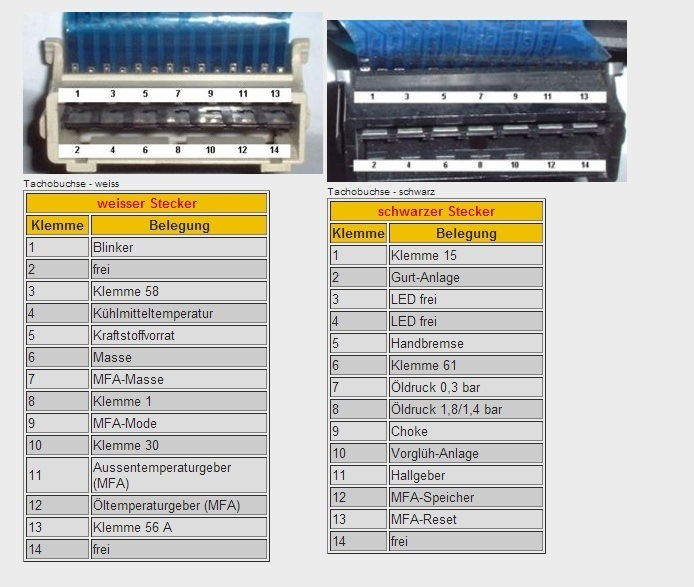
\includegraphics[width=0.72\textwidth]{digifiz_manual/image008.jpg}
    \caption{Disposition des connecteurs sur les tableaux \ReplicaGenOne{} à deux fiches.}
\end{figure}

\noindent\textbf{Connecteur blanc}

{\scriptsize
\begin{tblr}{
    colspec={Q[l,1.4cm] X[l]},
    hlines
}
\textbf{Broche} & \textbf{Affectation} \\
1 & Sortie clignotant, reliée à la masse pour le témoin lumineux. \\
2 & Frei --- non connecté. \\
3 & Borne~58, alimentation positive du rétroéclairage. \\
4 & Entrée de sonde de température de liquide de refroidissement résistive. \\
5 & Entrée de sonde de niveau de carburant résistive. \\
6 & Retour de masse. \\
7 & Retour de masse supplémentaire. \\
8 & Signal régime moteur borne~1 (bobine, distributeur ou autre forme jusqu'à 12~V avec des pics possibles à 300~V). \\
9 & Ligne de mode MFA utilisée pour changer les fonctions MFA. \\
10 & Alimentation permanente UNR (inutilisée sur \ReplicaGenOneShort{}, alimentation principale sur \ReplicaNextShort{}). \\
11 & Fil « + » de température MFA pour la sonde extérieure (\ReplicaNextShort{}). \\
12 & Fil de sonde de température d'huile MFA (\ReplicaNextShort{} uniquement). \\
13 & Entrée du témoin plein phare KL~56a (+12~V actif). \\
\end{tblr}}

\noindent\textbf{Connecteur noir}

{\scriptsize
\begin{tblr}{
    colspec={Q[l,1.4cm] X[l]},
    hlines
}
\textbf{Broche} & \textbf{Affectation} \\
1 & Borne~15, +12~V commuté depuis le contacteur d'allumage. \\
2--4 & Non connecté. \\
5 & Entrée du témoin de frein à main (actif à l'état bas). \\
6 & Pilotage de témoin d'alternateur KL~61 avec résistance d'excitation de 120~\ensuremath{\Omega}. \\
7 & Contact de pression d'huile 0,3~bar. \\
8 & Contact de pression d'huile 1,8~bar. \\
9 & Non utilisé. \\
10 & Entrée du témoin de préchauffage (+12~V actif, diesel uniquement). \\
11 & Entrée capteur Hall pour capteurs de vitesse optionnels. \\
12 & Ligne de sélection de bloc MFA. \\
13 & Ligne de remise à zéro MFA. \\
\end{tblr}}

\subsection{Blocs à connecteur unique}
Les tableaux à connecteur unique utilisent le câblage illustré à l'\autoref{fig:single-connector}.
Le faisceau reproduit les mêmes signaux que les variantes à deux connecteurs, mais les regroupe dans une seule fiche.

\begin{figure}[htbp]
    \centering
    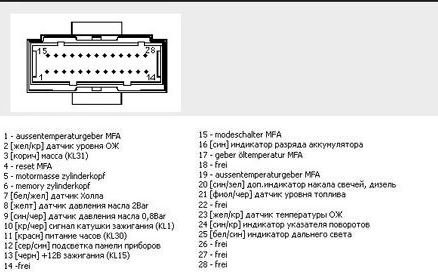
\includegraphics[width=0.65\textwidth]{digifiz_manual/image009.png}
    \caption{Disposition du connecteur unique utilisé sur les tableaux Replica compacts.}
    \label{fig:single-connector}
\end{figure}

\subsection{Faisceau prospectif Scirocco/Passat}
Le faisceau prospectif Scirocco/Passat utilise deux fiches.
Leurs fonctions sont résumées ci-dessous.

\noindent\textbf{Fiche 5~broches}
{\scriptsize
\begin{tblr}{
    colspec={Q[l,2.6cm] X[l]},
    hlines
}
\textbf{Broche} & \textbf{Affectation} \\
1~(D3) & Contact d'indication de gamme « D » de la boîte automatique. Met le témoin de conduite à la masse lorsque le sélecteur est en position~D. \\
2~(D2) & Contact d'indication de deuxième gamme de la boîte automatique. Met le témoin « 2 » à la masse lorsque le sélecteur est en position~2. \\
3~(D1) & Contact d'indication de première gamme de la boîte automatique. Met le témoin « 1 » à la masse lorsque le sélecteur est en position~1. \\
4~(SA) & Alimentation commune de l'affichage de sélecteur automatique (\emph{Schaltanzeige}); fournit le +12~V aux voyants de gamme. \\
5~(SPERRE) & Contact d'interverrouillage de démarrage provenant du sélecteur. Fermé en position parking ou point mort pour autoriser le démarrage. \\
\end{tblr}}

\noindent\textbf{Fiche 14~broches}
{\scriptsize
\begin{tblr}{
    colspec={Q[l,2.6cm] X[l]},
    hlines
}
\textbf{Broche} & \textbf{Affectation} \\
1~(KL~58) & Alimentation d'éclairage pour le rétroéclairage du panneau. \\
2~(MASS) & Retour de masse châssis. \\
3~(TANK) & Entrée jauge de carburant. \\
4~(TEMP) & Entrée sonde de température de liquide de refroidissement. \\
5~(KL~1) & Signal de régime moteur (borne~1). \\
6~(UHR) & +12~V permanent pour l'horloge et la sauvegarde mémoire. \\
7~(FERNL) & Entrée témoin plein phare. \\
8~(reserved) & Non connecté. \\
9~(OEL~1.8) & Contact de pression d'huile haute, 1,8~bar. \\
10~(CAT~VORGL(-)) & Entrée témoin de préchauffage catalyseur/diesel (actif bas). \\
11~(OEL~0.3) & Contact de pression d'huile basse, 0,3~bar. \\
12~(KL~61) & Témoin d'alternateur et alimentation d'excitation. \\
13~(KL~49a) & Alimentation combinée du témoin de clignotants. \\
14~(KL~15) & Alimentation +12~V commutée par l'allumage. \\
\end{tblr}}

\subsection{Correspondance des connecteurs Mk1}
Les véhicules Volkswagen Mk1 utilisent les affectations suivantes~:
\begin{enumerate}
    \item Alimentation d'éclairage et de feux de croisement.
    \item Masse MASSE~31.
    \item Émetteur de niveau de carburant TANK.
    \item Sonde de température TEMP.
    \item Signal de compte-tours KL~1.
    \item +12~V permanent UHR.
    \item Signal plein phare KL~56.
    \item Contact de pression d'huile (HAUTE) 1,8~bar.
    \item Contact de pression d'huile (BASSE) 0,3~bar.
    \item Témoin de préchauffage diesel.
    \item Entrée starter (non utilisée).
    \item Lampe génératrice KL~61.
    \item Entrée clignotant (gauche/droite combinés).
    \item Alimentation d'allumage KL~15.
\end{enumerate}
\begin{figure}[htbp]
    \centering
    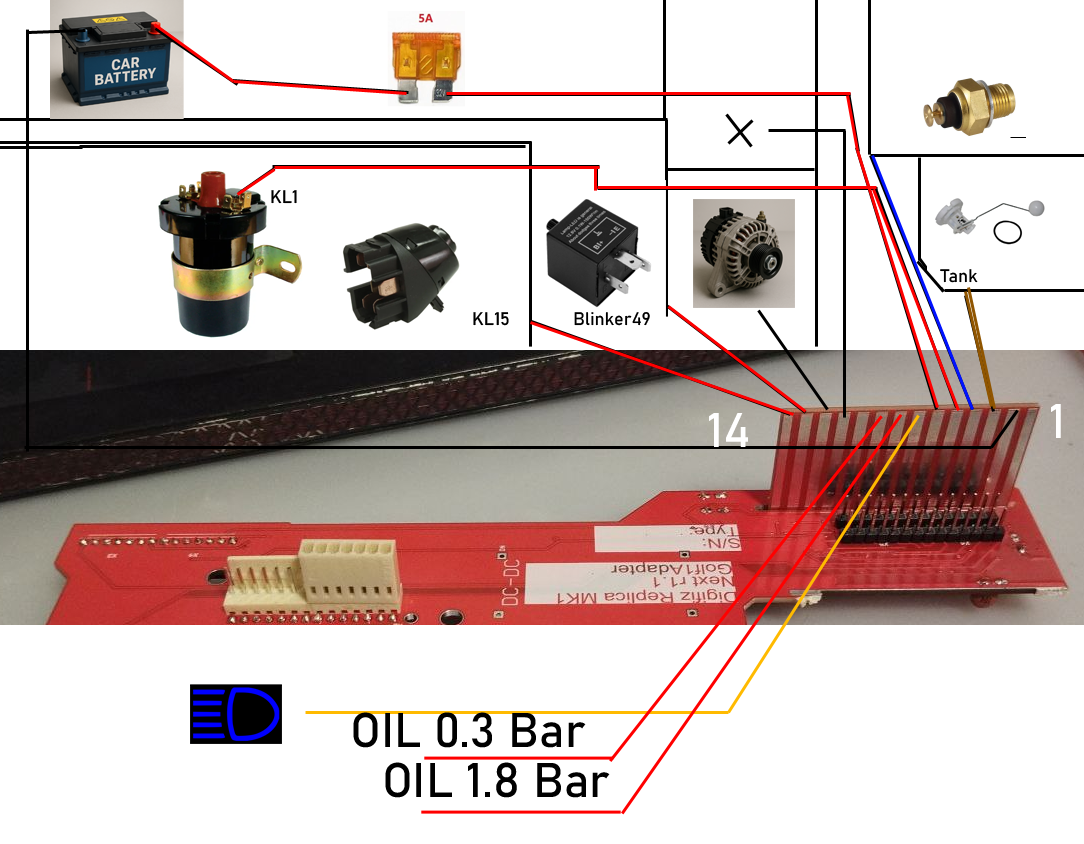
\includegraphics[width=0.75\textwidth]{digifiz_manual/image010.png}
    \caption{Schéma de connexion du faisceau pour les installations Mk1.}
\end{figure}

\subsection{Connecteur de service sur la carte}
Le troisième connecteur sur la carte reproduit les connecteurs du tableau, avec des broches numérotées de droite à gauche sur les unités \ReplicaGenOneShort{} et \ReplicaNextShort{}.
Il fournit une interface de service avec les affectations listées dans l'\autoref{tab:service-connector}.

\begin{table}[htbp]
    \centering
    \caption{Affectations des broches du connecteur de service.}
    \label{tab:service-connector}
    {\scriptsize
    \begin{tblr}{
        colspec={Q[l,1.9cm] X[l]},
        hlines,
    }
        \textbf{Position} & \textbf{Affectation} \\
        1 & Sortie témoin. \\
        2 & Entrée capteur de vitesse (SPM\_M). \\
        3 & Masse véhicule. \\
        4 & Sortie témoin. \\
        5 & Entrée optocoupleur clignotant gauche. \\
        6 & Entrée optocoupleur clignotant droit. \\
        7 & +12~V contact. \\
        8 & Entrée spécifique diesel. \\
        9 & Entrée témoin (positive). \\
        10 & Entrée régime alternative (inutilisée, \ReplicaNextShort{} uniquement). \\
        11 & \ReplicaGenOneShort{} : sortie témoin (normalement déconnectée) ; \ReplicaNextShort{} : entrée frein (active bas). \\
        12 & Réservé. \\
        13 & Entrée voyant moteur. \\
        14 & Aucun contact. \\
    \end{tblr}}
\end{table}

\subsection{Connecteurs d'extension auxiliaires}
Trois barrettes supplémentaires à quatre broches sont montées sur la carte principale pour faciliter les évolutions de faisceau et les opérations de service~:
\begin{itemize}
    \item \textbf{Signaux analogiques d'extension~:} offre un accès dédié pour ajouter des entrées analogiques lors de l'intégration de capteurs personnalisés.
    \item \textbf{Miroir MFA~:} duplique le connecteur \textsc{MFA} standard pour permettre un piquage parallèle des signaux de l'ordinateur de bord.
    \item \textbf{Doublons analogiques~:} répète les entrées température d'huile, température ambiante et témoin de frein afin de les router vers des modules de journalisation ou de surveillance externes.
\end{itemize}
Les trois utilisent le connecteur femelle \mbox{KF2510-4p}, non fourni avec le kit tableau de bord et à se procurer séparément si nécessaire.

\begin{figure}[htbp]
    \centering
    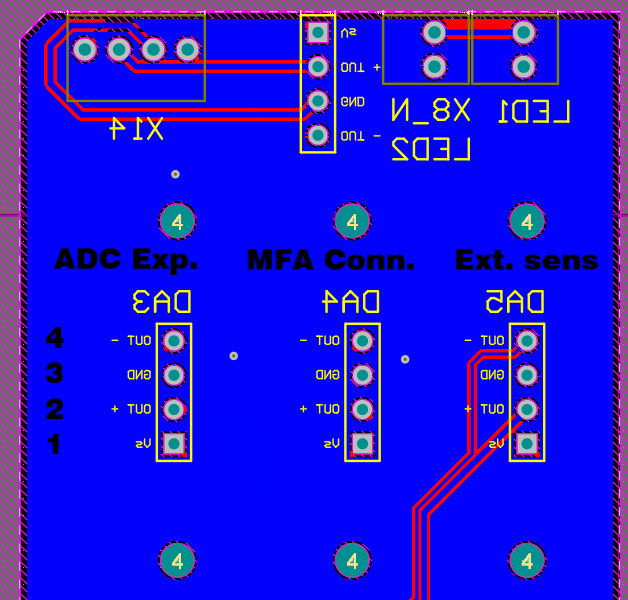
\includegraphics[width=0.6\textwidth]{digifiz_manual/ext_conn.png}
    \caption{Disposition des connecteurs auxiliaires sur la carte principale.}
\end{figure}

\begin{table}[htbp]
    \centering
    {\small
    \begin{tblr}{
        colspec={Q[l,2.3cm] Q[c,1.3cm] X[l]},
        hlines,
        row{1} = {font=\bfseries}
    }
    Connecteur & Broche & Affectation \\
    Connecteur~I & 4 & Entrée analogique auxiliaire~1 \\
    Connecteur~I & 3 & Masse (GND) \\
    Connecteur~I & 2 & Entrée analogique auxiliaire~2 \\
    Connecteur~I & 1 & VCC (3V3, non protégée\textbf{!!!}) \\
    Connecteur~II & 4 & Remise à zéro MFA \\
    Connecteur~II & 3 & Masse (GND) \\
    Connecteur~II & 2 & Bloc mémoire MFA \\
    Connecteur~II & 1 & Mode MFA \\
    Connecteur~III & 4 & Sortie sonde de température d'huile \\
    Connecteur~III & 3 & Masse (GND) \\
    Connecteur~III & 2 & Sortie sonde de température extérieure \\
    Connecteur~III & 1 & Témoin de frein \\
    \end{tblr}}
    \caption{Affectations des connecteurs d'extension auxiliaires.}
\end{table}

\section{Logiciel embarqué et contenu}
Le micrologiciel du tableau de bord est publié à l'adresse suivante~:
\displayurl{https://github.com/Sgw32/DigifizReplica}
Deux ensembles de livraison sont disponibles~:
\begin{itemize}
    \item \textbf{\ReplicaGenOne{}~:} tableau de bord, faisceau de température d'air et d'huile, programmateur USBasp et, pour les capteurs déportés, faisceau de capteur de vitesse.
    \item \textbf{\ReplicaNextLong{}~:} tableau de bord et faisceau pour capteur de vitesse électronique.
\end{itemize}
